\chapter{Model validation} \label{ch:6}
Making changes in the way of flying is quite dangerous with a quadcopter. These changes can namely cause unstability resulting in a crash. Hence, modeling the behaviour of a quadcopter can be of great addition. The Ardupilot code is transformed into a simulink model and simplified, so that it is more userfriendly. Because of the complexity of the Ardupilot code, it is very difficult to make changes. Thereby is taken into account that the dynamics are still according the rules of nature. Controllers, observers and routeplanning can now be tested in a more controllable environment. \\

\section{Build up}
Starting with the Equations of motion, explained in Chapter \ref{ch:3}. The plant is created by a six D.O.F. block that basically gives all the required outputs, calculated from the incoming moments, forces and current states. Parts of the 
To simulate reality, the simulink model is created as real as possible, including measurement and process noise and other affects as well. Changes in the system can be made by validating the directions and there is even a possibility to add the motormixer if required. However, this is excluded for the rest of this report to simplify the system. Including this motormixer will be stable with retuning the control parameters.\\

Furthermore is the position controller also implemented. This is another flying mode, different from the Stabilize mode explained in Chapter \ref{ch:4}, namely Auto. This implementation requires more than the inner Rate loop, since has not direct influence into the plant, but outputs desired angular rates. Consequently, it does not use the previous attitude controller anymore, but has this included in the horizontal error angle controller. This challenge can be solved in various ways, but the Moller's [2 Moller] method. The control scheme is also visualised in Figure \ref{fig:positionreference}. 

\begin{figure}[H]
\centering
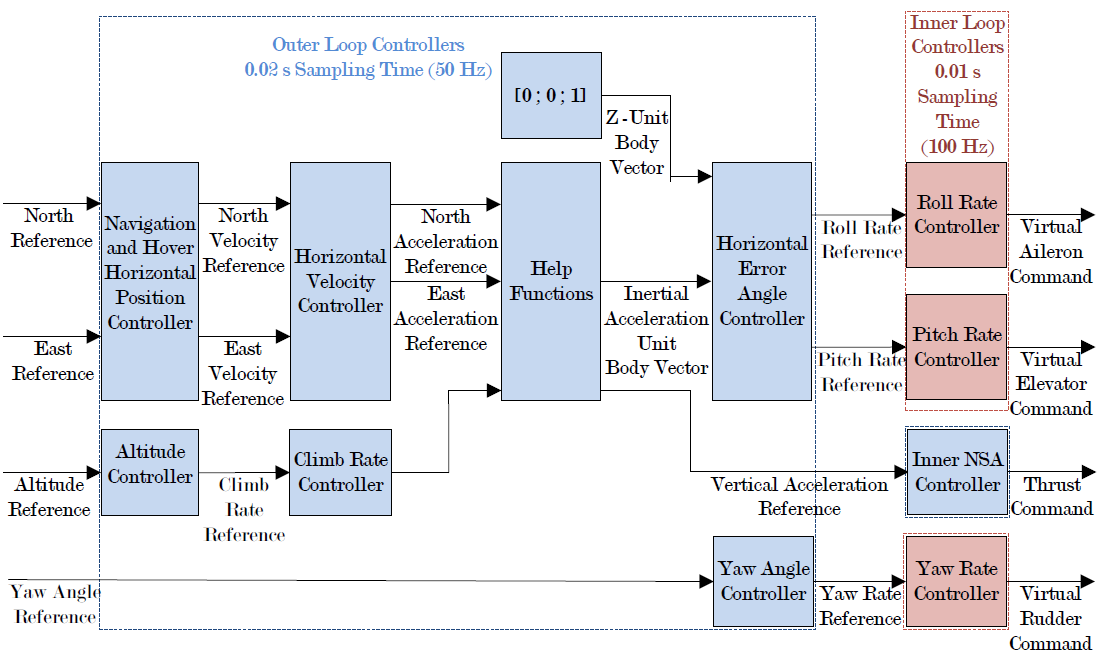
\includegraphics[width=0.9\textwidth]{positionreference.png}
\caption{Moment vs wall gap (square marker: moments about y-axis; circle marker: moments about x-axis).}
\label{fig:positionreference}
\end{figure}

Note that yaw control is completely seperate from pitch and roll. Yaw control is seperate, because of roll and pitch are prioritised for stable hovering. The block helping functions consists of... \textcolor{red}{HIER NOG AANVULLEN. ook bijvoegen met acceleratie vector blabla}.

\section{Comparison}
Since there is no obtained flightdata for now, the model still has to be verified. However, the created model constists of a lot of details, besides the equations of motion. The model in personalized in the matter of the following list: Inertia, geometry, Thrust-profiles, vibrations and mass. There is assumed that the drone repesents reality eventhough the real validation cannot be done. This is already been proved by  research in the past. \textcolor{red}{Hier nog bronnen bijgeven dat drones goed the modeleren zijn}\\

\section{Near-wall effect}
There are two different effects that occur when flying close to a wall caused by airflow. Because of a not uniformly distributed thrust over the propeller there are extra moments working upon the propeller [1 near wall paper]. Additionally, the airflow not being able to have sufficient instream causing the propeller to lose some thrust. The thrust losses are obtained by experiments, which are discussed Chapter \ref{Ch:33}. For the external moments caused by the not uniformly distributions of air flow are calculated by scaling the moments with the following non-dimensionalised moment.
\begin{equation}
M^{*}= \frac{M}{WG mg}
\end{equation}

With $M^{*}$ as non-dimensionalised moment, $M$ moment, $WG$ wallgap distance. The results from the numerical simulation from [1 Near wall effect] are shown in Figure \ref{fig:nearwall}.

\begin{figure}[H]
\centering
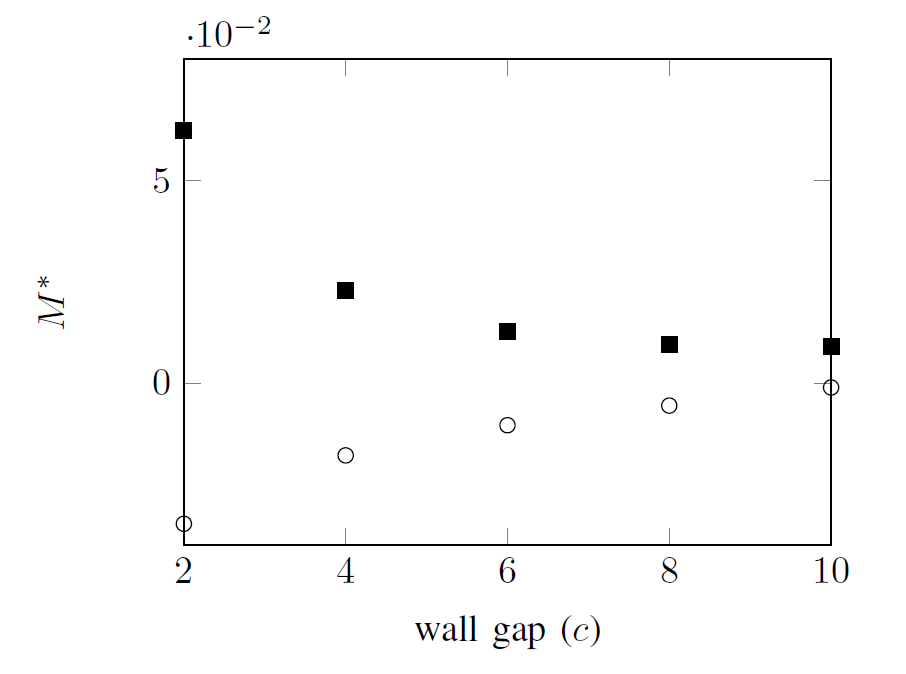
\includegraphics[width=0.5\textwidth]{nearwallgraph.PNG}
\caption{Moment vs wall gap (square marker: moments about y-axis; circle marker: moments about x-axis).}
\label{fig:nearwall}
\end{figure}

The result that is shown in Figure \ref{fig:nearwall} can be used with scaling $M^{*}$ to $M$ and are implemented.\\
\textcolor{red}{Extra information about the not uniformly distribution over the propeller. $https://www.mathworks.com/videos/programming-drones-with-simulink-1513024653640.html$}

\subsection{Implementation} \label{Ch:33}
As mentioned before, the implementation of the disturbance is seen as a thrustloss of one of the motors and an extra moment upon the quadcopter. Because of this significantly big sudden effect on the drone, it is not controllable by a simple PID-controller. Consequently, other techniques should be used to counter sudden effect.\\

Three options:
\begin{itemize}
\item Very agressive controller.\\
\item Feed forward. \\
\item Disturbance observer could be designed.\\
\url{http://ieeexplore.ieee.org/stamp/stamp.jsp?arnumber=6842357} see the discussion to see approach how to make a disturbance observer.\\
\end{itemize}

Disturbance Observer Based Control (DOBC) is hereby tried to account for the near-wall effects. The basic idea of DOBC is estimating the disturbance (or effects caused by it) from measured variables and control that observed disturbance to compensate for the influence of the disturbance. Normally the DOBC is used independently of the tracking control. DOBC is benificial that it uses no extra sensors to detect the disturbance, but tries to observe it. The disturbance observer should moreover not interfere with the tracking control. The system could get unstable if the influence is too big.\\



\textcolor{red}{Hier plaatjes van de disturbance in het system implementation en uitleg}\\ 